\documentclass[12pt,notitlepage]{article}
\author{Leo Przybylski \\
\texttt{przybyls@arizona.edu}}
\usepackage{listings}
\usepackage{color}
\usepackage{graphicx}

\title{Change Promotion Environment Flow}

\begin{document}
\maketitle
\tableofcontents

\lstset{basicstyle=\small,
  breaklines=true,
  includerangemarker=false}

\abstract{The flow of code in any given state needs to be illustrated and described in 
detail as it goes from environment to environment. There are a number of different scenarios
that can be discovered through change promotion. Each scenario has been explored
and illustrated with steps. Scenarios also have a number of exceptional cases that
may occur. Those have also been explored.}

\section{Overview and Goals}
\subsection{Goals}
\begin{itemize}
\item State breakdown as code transitions from environment to environment
\item Illustration of change promotion for the following scenarios:
  \begin{itemize}
  \item Emergency bug fix
  \item Normal change
  \item Bug fix
  \end{itemize}
\end{itemize}

\section{Emergency Bug Fix}
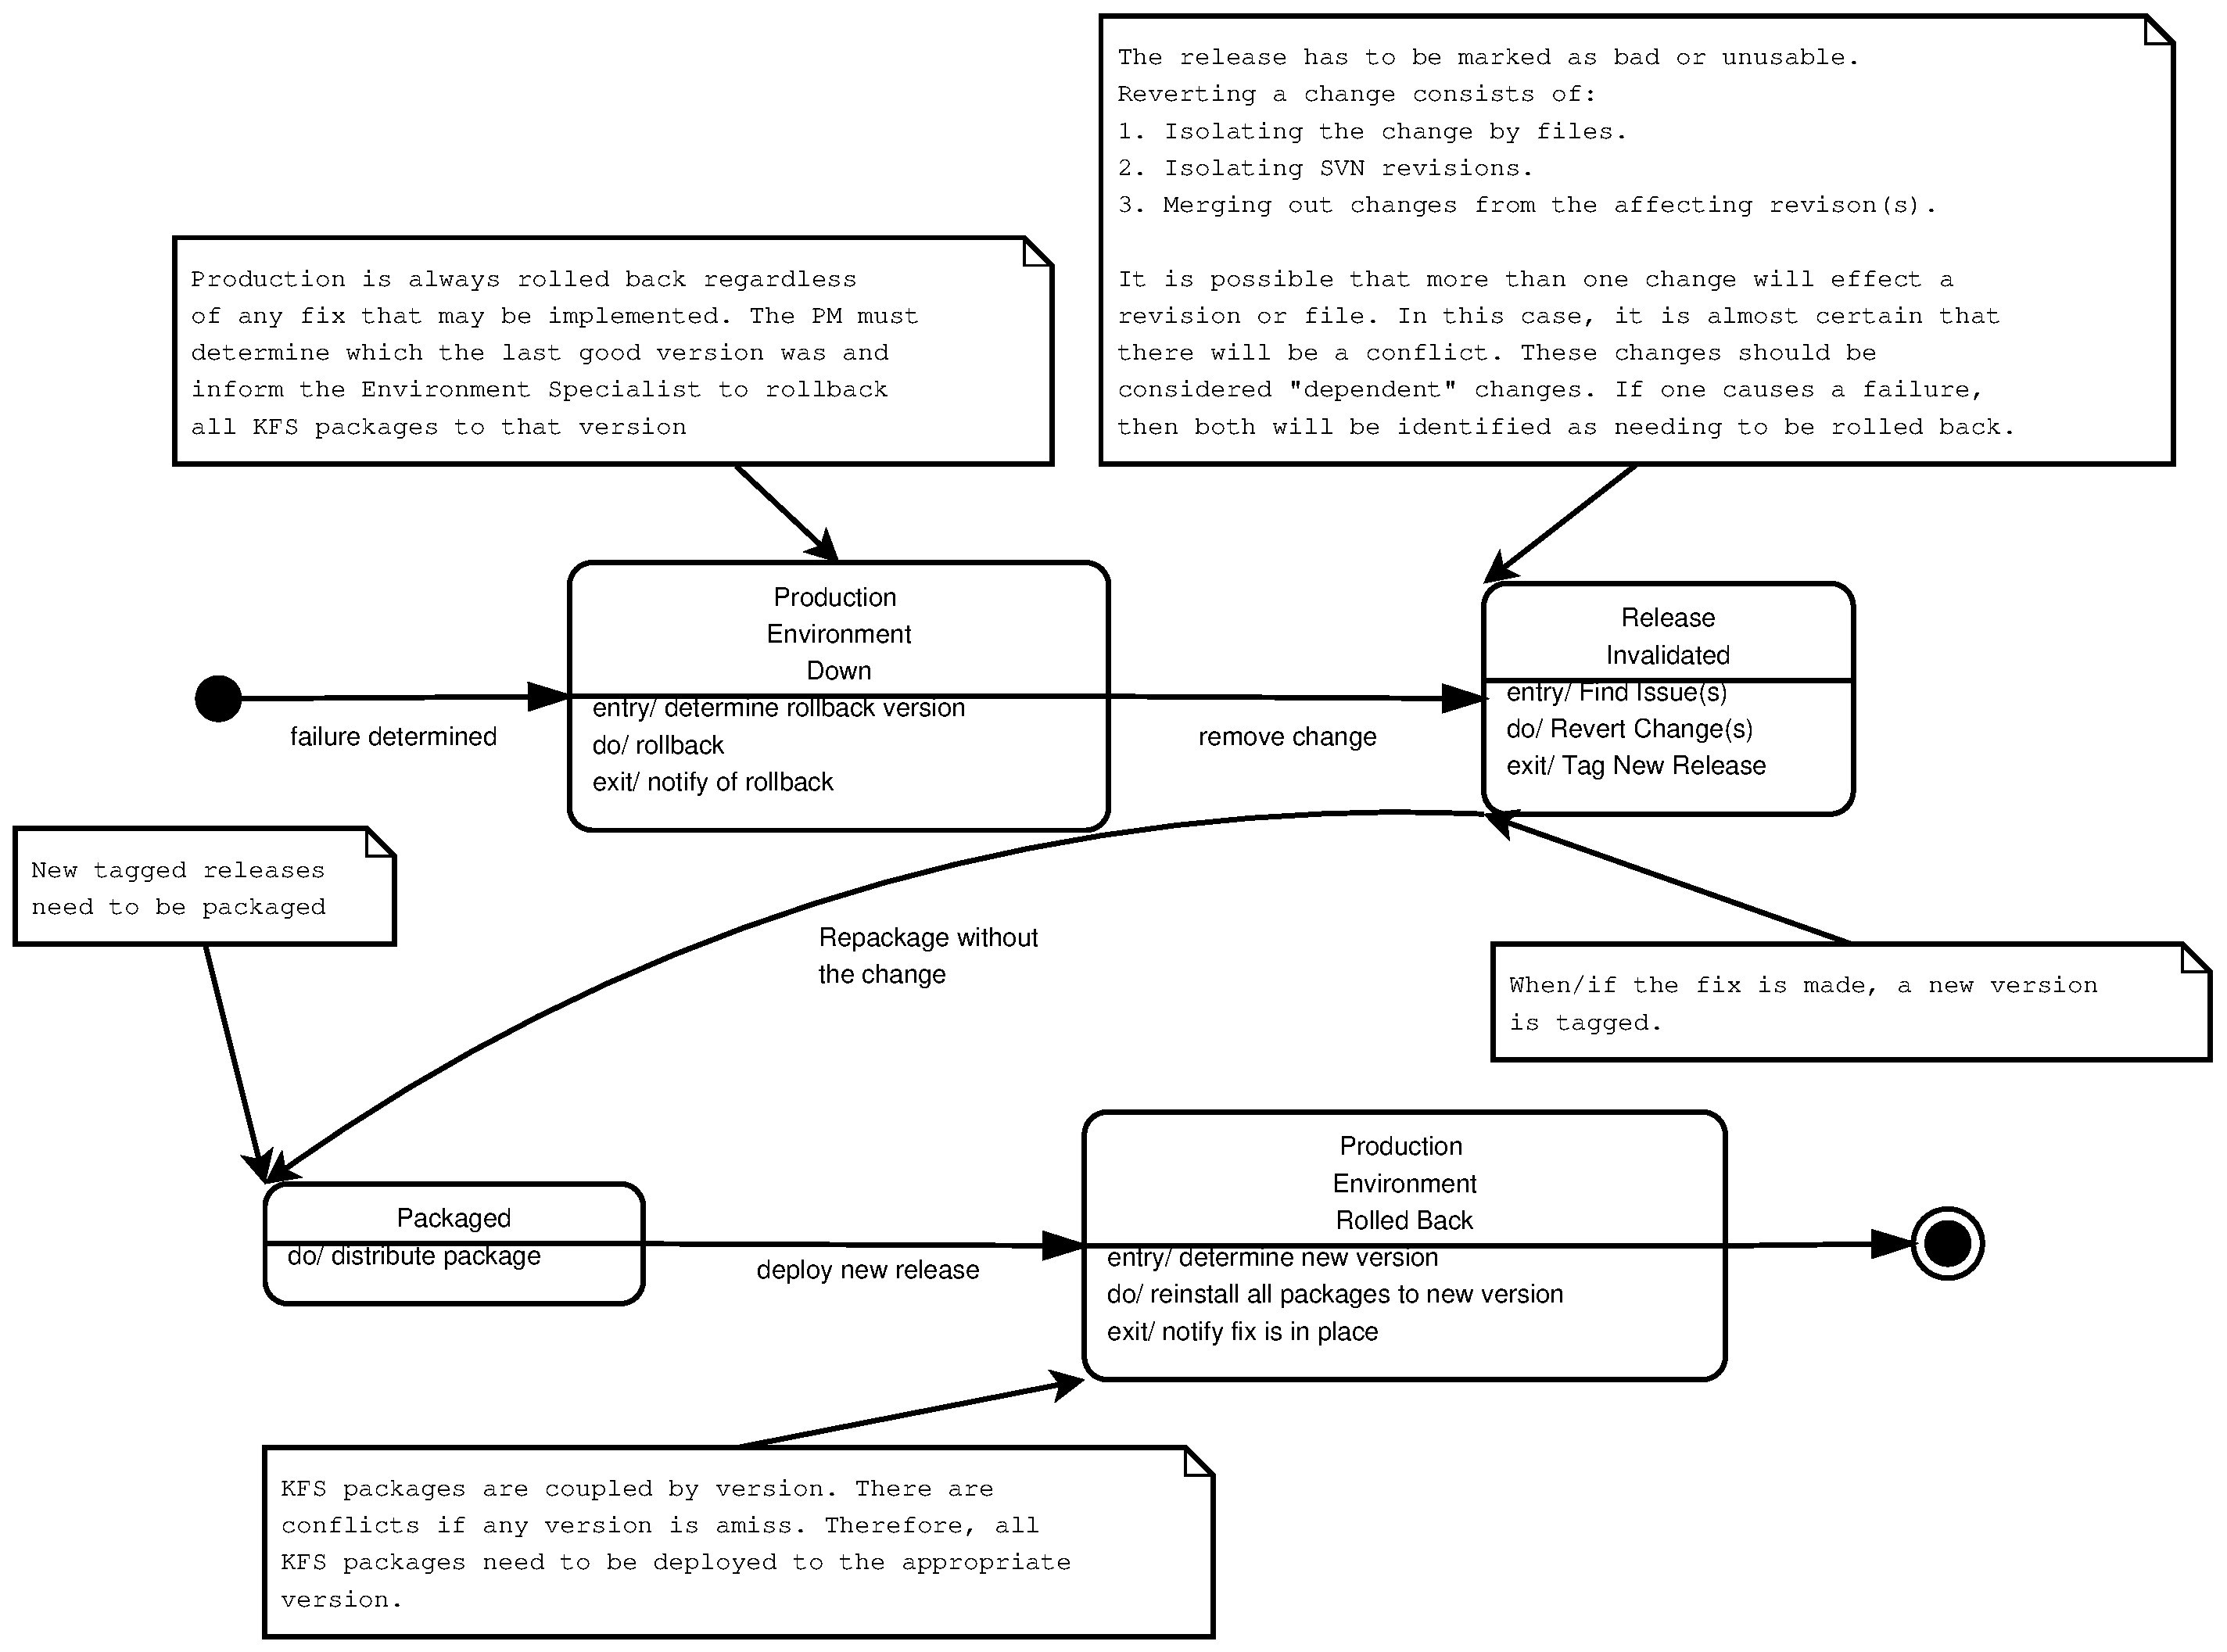
\includegraphics[width=12cm]{Diagrams/ChangePromotion_State2.eps}
\subsection{Change has Broken the Application Without Dependencies}

\subsubsection{Actors}
\emph{These actors are not official roles. That is a person can be considered to
participate in all of these roles. For example, if there is no such thing as a Configuration
Manager in the project, then a Developer may be filling that role. For the sake of
this document, the roles are exclusively identified.}
\begin{itemize}
\item Developer
\item Configuration Manager
\item Project Manager
\item Environment Specialist
\end{itemize}

\subsubsection{Steps}
\begin{enumerate}
\item Developer determines the problem and notifies the Project Manager
\item Project Manager informs Configuration Manager to pull the change.
\item Configuration Manager locates Jira issue related to change.
\item Configuration Manager merges changes back to the development branch for fixing the bug.
\item Configuration Manager determines revisions for the change.
\item Configuration Manager determines files effected by change.
\item Configuration Manager reverts by revision each file effected. \emph{Note: there are no dependencies
  on files, so we can assume that these files do not effect other changes.}
\item Configuration Manager tags a new release.
\item Configuration Manager begins an ad hoc run of packaging process.
\item Configuration Manager notifies the Project Manager the fix is ready.
\item Project Manager notifies an Environment Specialist to deploy the fix.
\item Environment Specialist deploys the fix to SUP.
\item Environment Specialist notifies Project Manager of deployment.
\item Project Manager notifies tester to test.
\item Tester notifies Project Manager status is good.
\item Project Manager notifies Environment Specialist to deploy to PROD.
\end{enumerate}

\subsection{Change has Broken the Application With Dependencies}
\subsubsection{Actors}
\emph{These actors are not official roles. That is a person can be considered to
participate in all of these roles. For example, if there is no such thing as a Configuration
Manager in the project, then a Developer may be filling that role. For the sake of
this document, the roles are exclusively identified.}
\begin{itemize}
\item Developer
\item Configuration Manager
\item Project Manager
\item Environment Specialist
\item Tester
\end{itemize}

\subsubsection{Steps}
\begin{enumerate}
\item Developer determines the problem and notifies the Project Manager
\item Project Manager informs Configuration Manager to pull the change.
\item Configuration Manager locates Jira issue related to change.
\item Configuration Manager merges changes back to the development branch for fixing the bug.
\item Configuration Manager determines revisions for the change.
\item Configuration Manager determines files effected by change.
\item Configuration Manager manually merges changes and resolves conflicts with dependencies. If 
  dependencies cannot be disconnected then
  \begin{enumerate}
    \item Configuration Manager gathers dependent issues.
    \item Configuration Manager reports dependent issues to Project Manager.
    \item Project Manager instructs Configuration Manager to remove dependent issues.
    \item Configuration Manager starts at step 1.
  \end{enumerate}
\item Configuration Manager tags a new release.
\item Configuration Manager begins an ad hoc run of packaging process.
\item Configuration Manager notifies the Project Manager the fix is ready.
\item Project Manager notifies an Environment Specialist to deploy the fix.
\item Environment Specialist deploys the fix to SUP.
\item Environment Specialist notifies Project Manager of deployment.
\item Project Manager notifies tester to test.
\item Tester notifies Project Manager status is good.
\item Project Manager notifies Environment Specialist to deploy to PROD.
\end{enumerate}

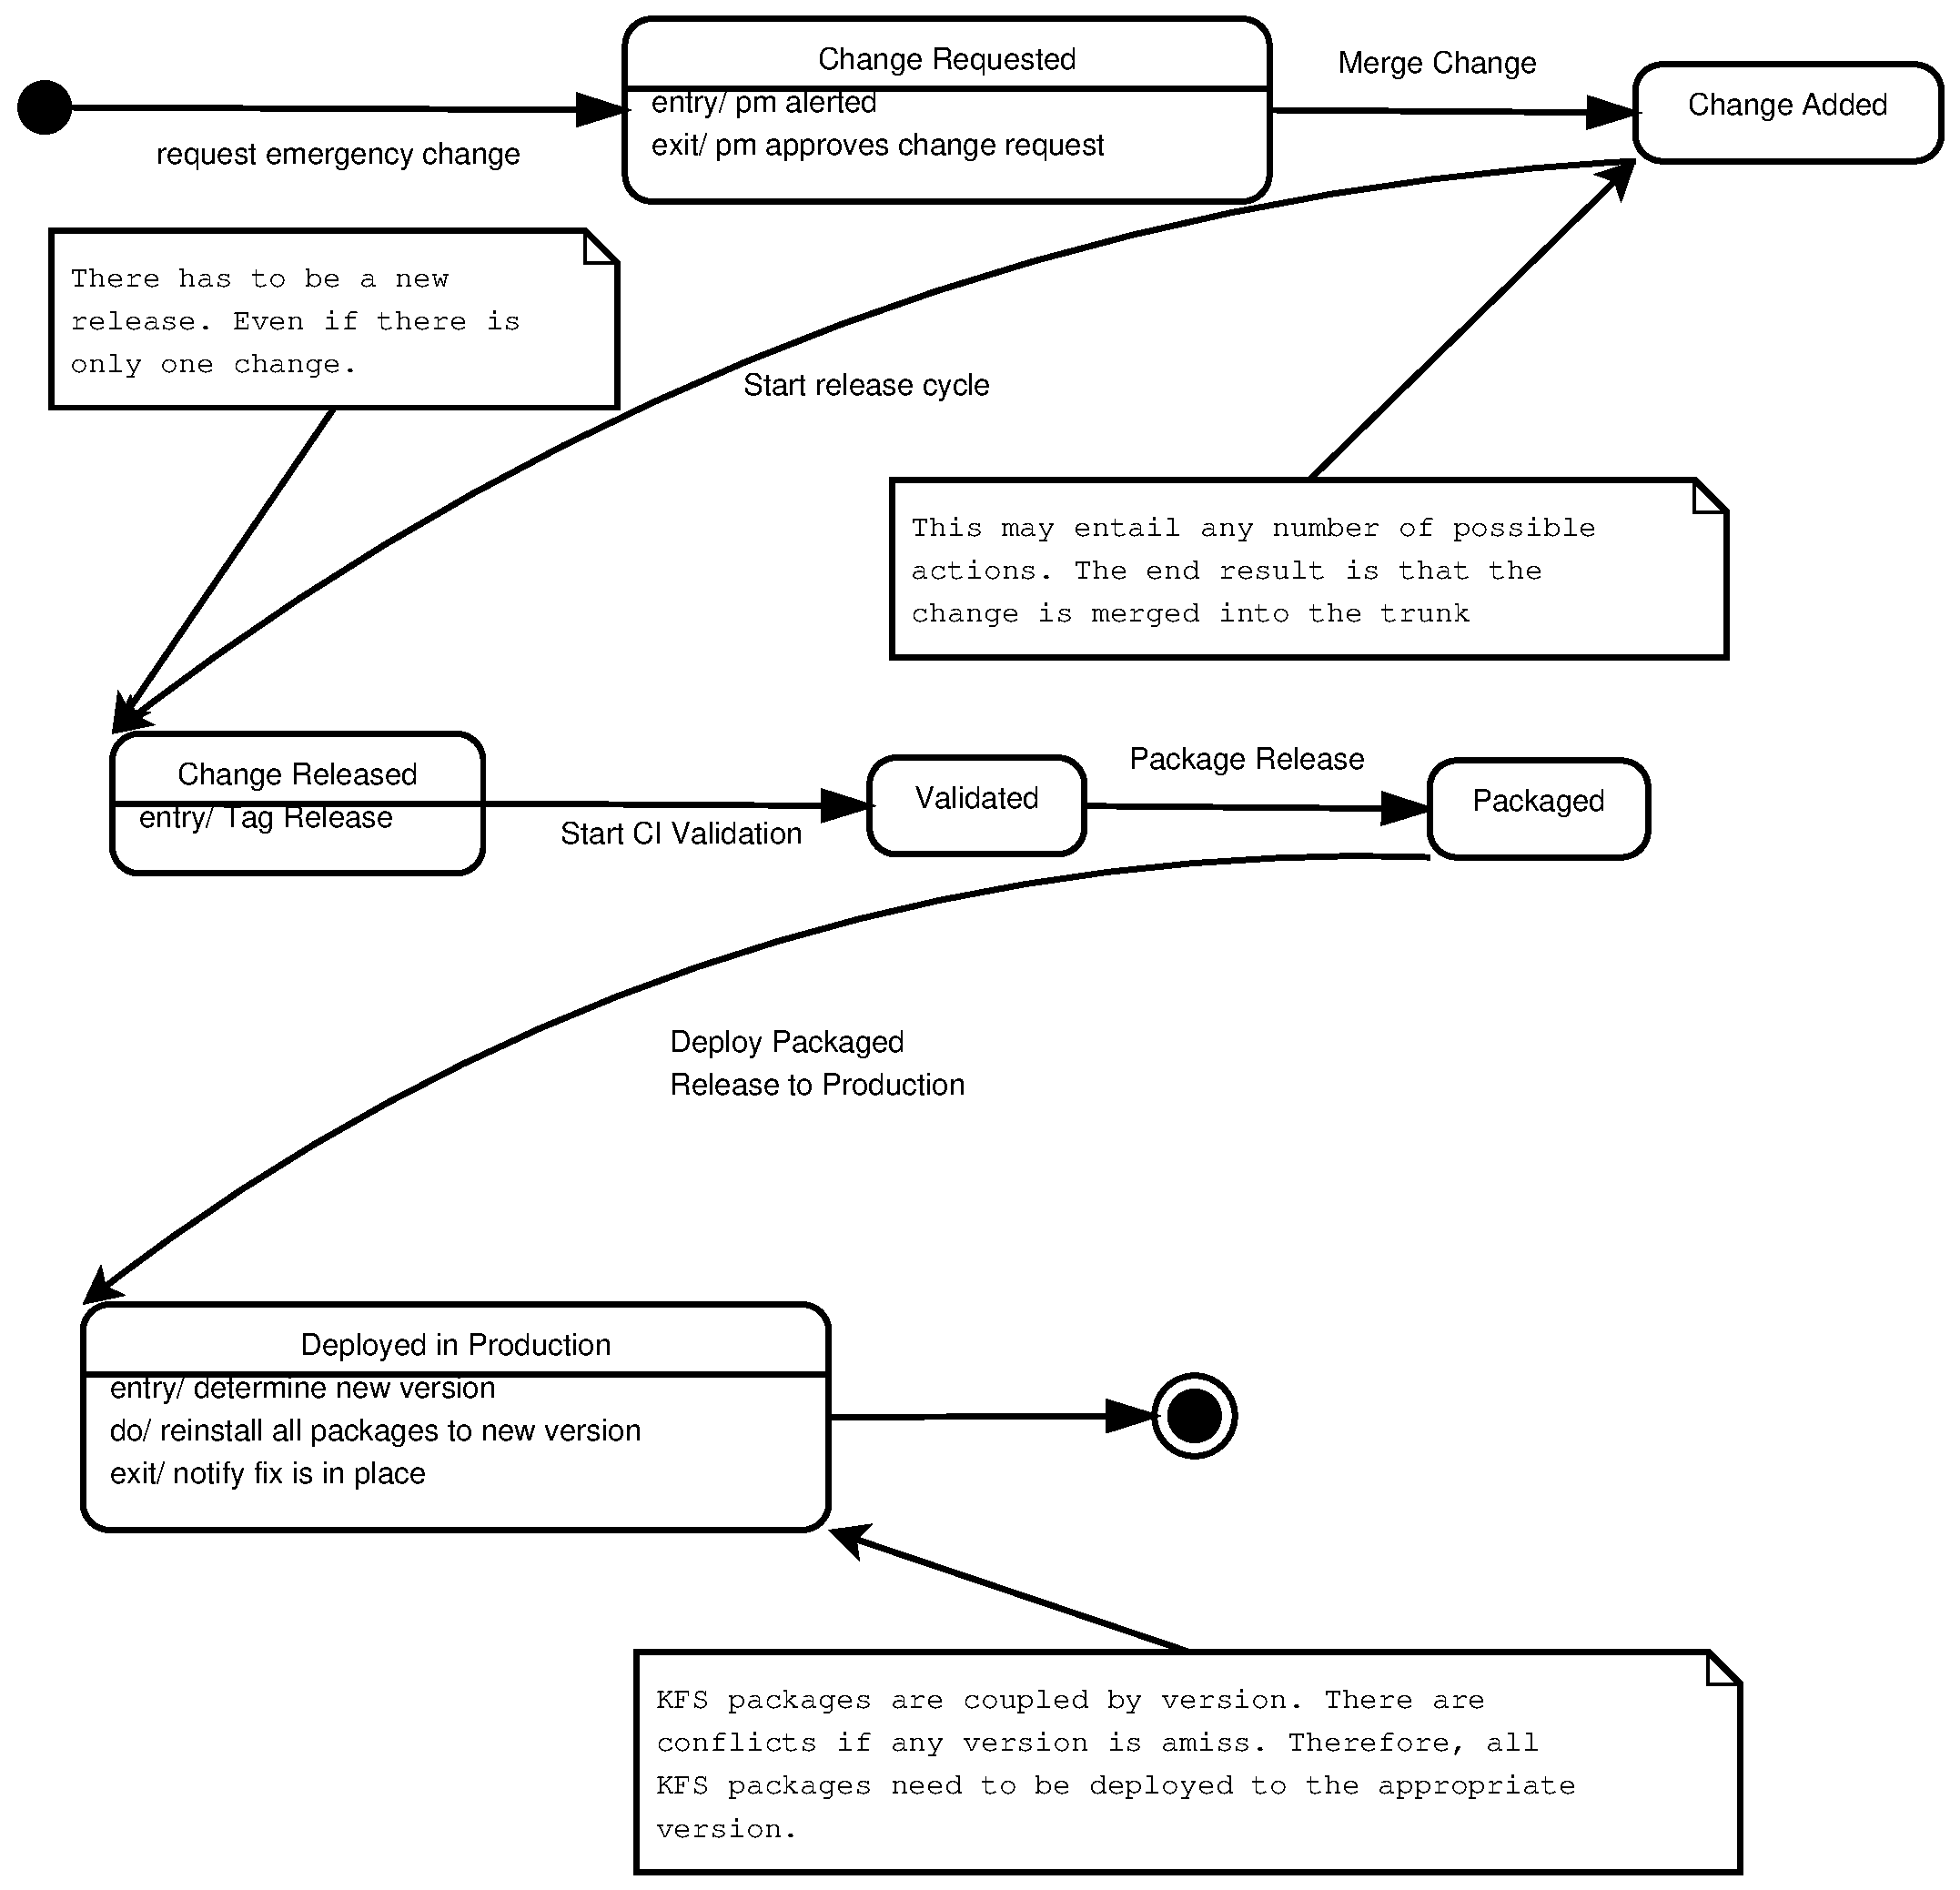
\includegraphics[width=12cm]{Diagrams/ChangePromotion_State3.eps}
\subsection{Need to Push New Code Change}
\subsubsection{Actors}
\emph{These actors are not official roles. That is a person can be considered to
participate in all of these roles. For example, if there is no such thing as a Configuration
Manager in the project, then a Developer may be filling that role. For the sake of
this document, the roles are exclusively identified.}
\begin{itemize}
\item Developer
\item Configuration Manager
\item Project Manager
\item Environment Specialist
\end{itemize}

\subsubsection{Steps}
\begin{enumerate}
\item Developer alerts Project Manager of new emergency change.
\item Developer merges new change into trunk.
\item Project Manager informs Configuration Manager to push new change.
\item Configuration Manager tags a new release.
\item Configuration Manager begins an ad hoc run of packaging process.
\item Configuration Manager notifies the Project Manager the fix is ready.
\item Project Manager notifies an Environment Specialist to deploy the fix.
\item Environment Specialist deploys the fix to SUP.
\item Environment Specialist notifies Project Manager of deployment.
\item Project Manager notifies tester to test.
\item Tester notifies Project Manager status is good.
\item Project Manager notifies Environment Specialist to deploy to PROD.
\end{enumerate}

\subsection{Exceptions}
\subsubsection{Not all changes are marked with the Jira issue \#}
This can be a problem if a developer checks in code and fails to either assign
a Jira \# or the correct Jira \#. Giving an incorrect Jira \# can have really
bad consequences in this scenario.

\subsubsection{Multiple issues were merged at one time}
Issues will have to be merged one at a time to avoid conflicts. If any issues are merged
together that have dependent files, then this may cause some confusion. It is better
to merge one at a time if possible.

\subsubsection{Different issues in merge update the same file and cause conflicts on rollback}

\section{Normal Change}
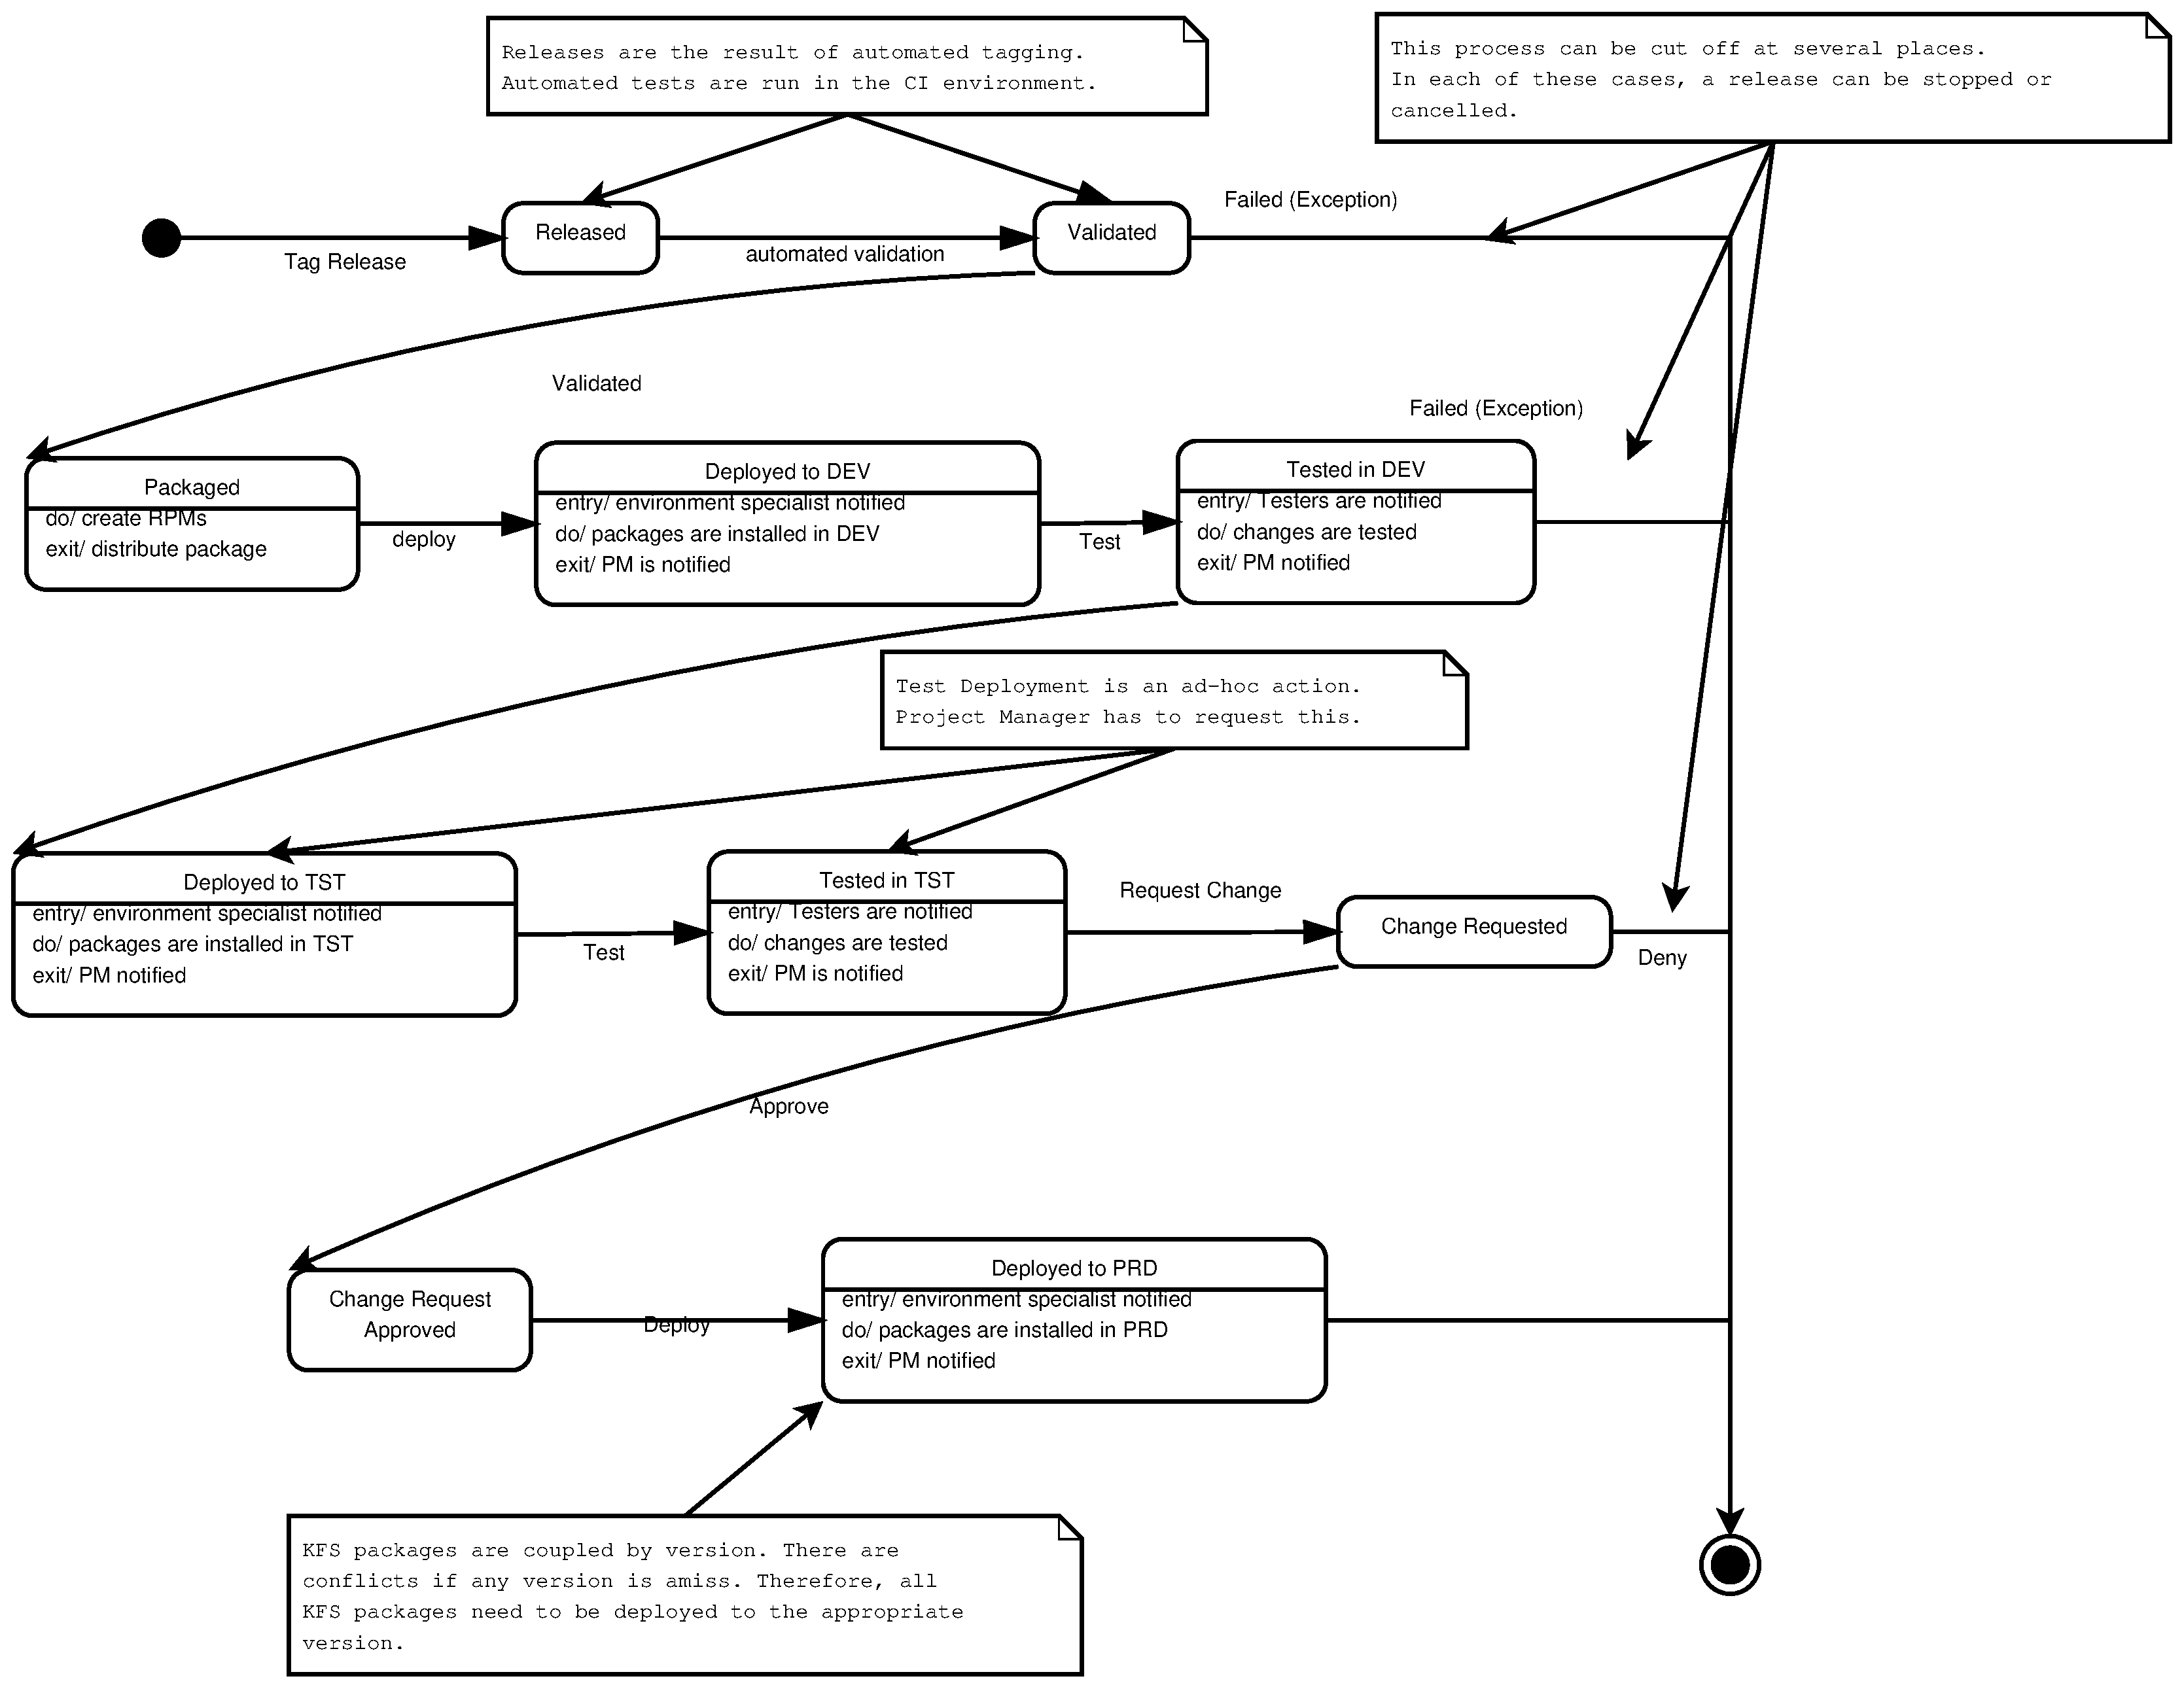
\includegraphics[width=12cm]{Diagrams/ChangePromotion_State4.eps}
In this scenario, changes are collected into a \emph{Release}. An entire \emph{Release} is to be
developed, tested, approved, and promoted. A \emph{Release} is composed of individual changes. If
any changes is not approved, then neither is a \emph{Release}.

\subsection{Actors}
\emph{These actors are not official roles. That is a person can be considered to
participate in all of these roles. For example, if there is no such thing as a Configuration
Manager in the project, then a Developer may be filling that role. For the sake of
this document, the roles are exclusively identified.}
\begin{itemize}
\item Configuration Manager
\item Project Manager
\item Environment Specialist
\item Tester
\end{itemize}

\subsection{Steps}
\begin{enumerate}
  \item Configuration Manager tags a release.
  \item Configuration Manager initiates testing and validation of release.
  \item Configuration Manager starts packaging of release.
  \item Configuration Manager notifies Environment Specialist that package is ready.
  \item Environment Specialist deploys release to DEV.
  \item Project Manager notifies Tester to checkout release in DEV.
  \item Tester tests release in DEV.
  \item Tester notifies Project Manager that DEV looks good.
  \item Project Manager determines that the release in DEV is valid.
  \item Project Manager notifies Environment Specialist to deploy release in DEV to TST.
  \item Environment Specialist deploys release in DEV to TST.
  \item Environment Specialist notifies Project Manager.
  \item Project Manager notifies Tester to test release in TST.
  \item Tester tests release in TST.
  \item Tester notifies Project Manager that TST looks good.
  \item Project Manager determines that the release in TST is valid.
  \item Project Manager submits formal change request for PROD.
  \item Change request is approved.
  \item Project Manager notifies Environment Specialist to deploy the approved release to PROD.
  \item Environment Specialist deploys the approved release to PROD.
  \item Environment Specialist notifies Project Manager that deployment to PROD was successful.
\end{enumerate}

\section{Bug fix}
\subsection{Actors}
\emph{These actors are not official roles. That is a person can be considered to
participate in all of these roles. For example, if there is no such thing as a Configuration
Manager in the project, then a Developer may be filling that role. For the sake of
this document, the roles are exclusively identified.}
\begin{itemize}
  \item Project Manager
  \item Developer
  \item Tester
  \item Configuration Manager
\end{itemize}

\subsection{Steps}
\begin{enumerate}
  \item Configuration Manager tags a release.
  \item Configuration Manager initiates testing and validation of release.
  \item Configuration Manager starts packaging of release.
  \item Configuration Manager notifies Environment Specialist that package is ready.
  \item Environment Specialist deploys release to DEV.
  \item Project Manager notifies Tester to checkout release in DEV.
  \item Tester tests release in DEV.
  \item Tester notifies Project Manager that DEV looks good.
  \item Project Manager determines that the release in DEV is valid.
  \item Project Manager notifies Environment Specialist to deploy release in DEV to TST.
  \item Environment Specialist deploys release in DEV to TST.
  \item Environment Specialist notifies Project Manager.
  \item Project Manager notifies Tester to test release in TST.
  \item Tester tests release in TST.
  \item Tester notifies Project Manager that TST looks good.
  \item Project Manager determines that the release in TST is valid.
  \item Project Manager submits formal change request for PROD.
  \item Change request is approved.
  \item Project Manager notifies Environment Specialist to deploy the approved release to PROD.
  \item Environment Specialist deploys the approved release to PROD.
  \item Environment Specialist notifies Project Manager that deployment to PROD was successful.
\end{enumerate}

\section{Exception}
\subsection{Change Did Not Pass DEV Environment Validation}
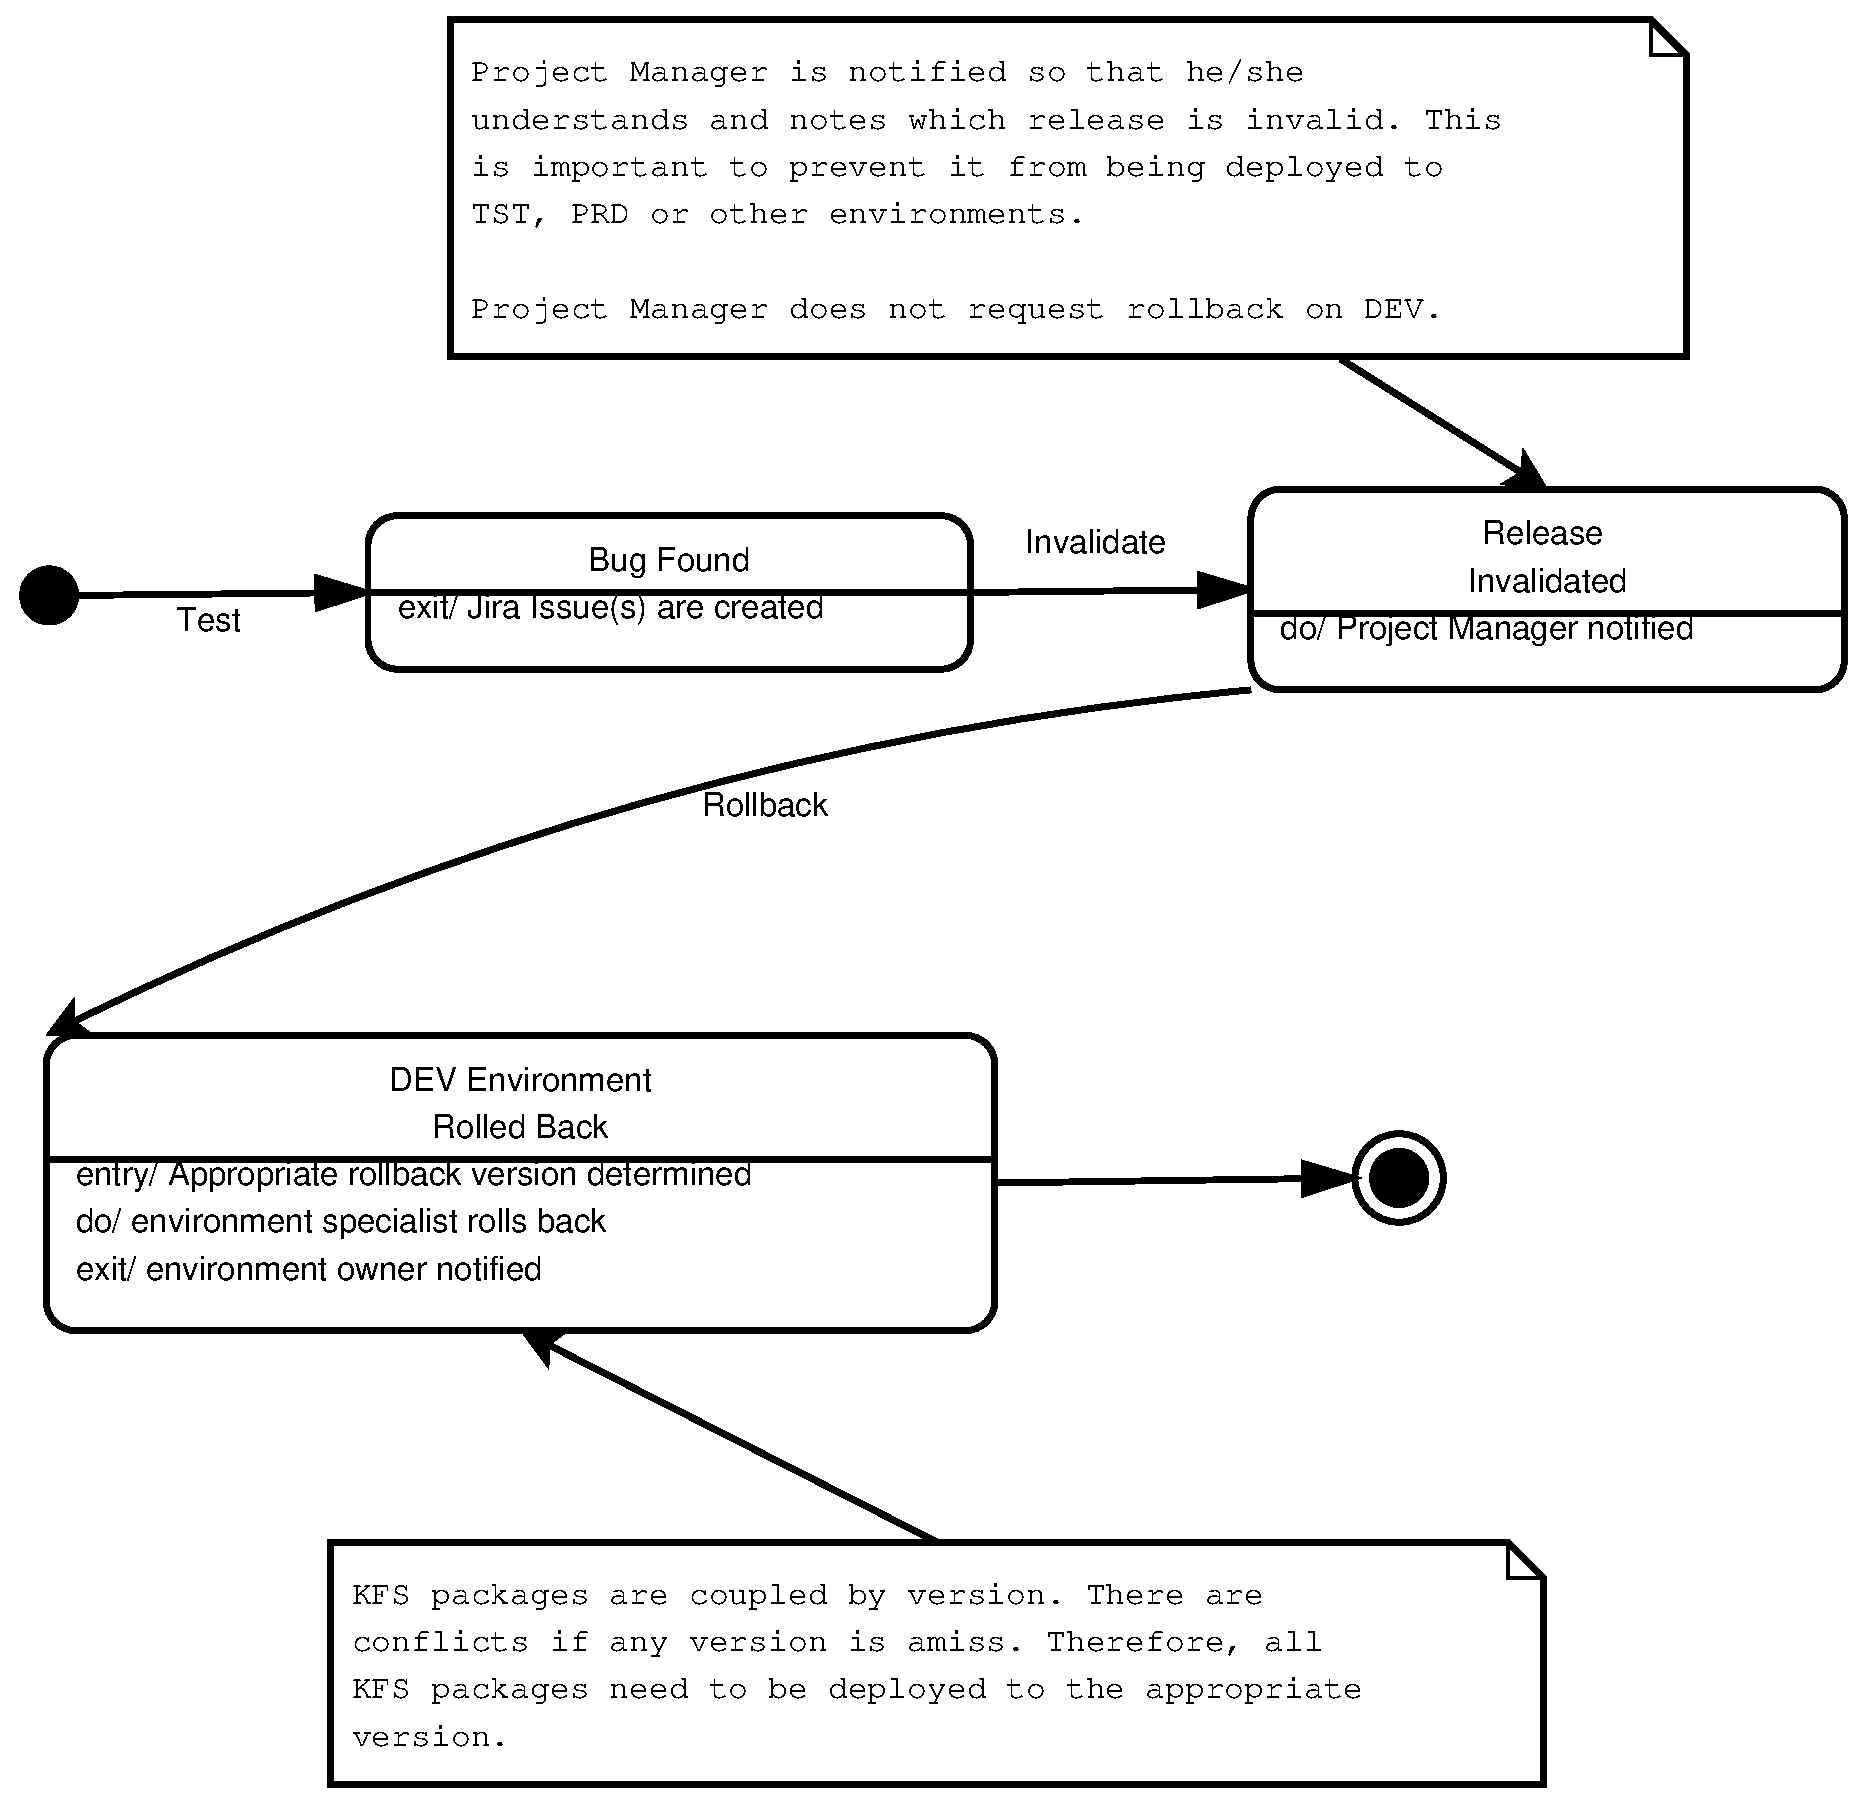
\includegraphics[width=12cm]{Diagrams/ChangePromotion_State5.eps}
\subsubsection{Actors}
\emph{These actors are not official roles. That is a person can be considered to
participate in all of these roles. For example, if there is no such thing as a Configuration
Manager in the project, then a Developer may be filling that role. For the sake of
this document, the roles are exclusively identified.}
\begin{itemize}
  \item Project Manager
  \item Developer
  \item Tester
  \item DEV Environment Owner
  \item Configuration Manager
\end{itemize}

\subsubsection{Steps}
\begin{enumerate}
  \item Tester is notified of ready build in DEV.
  \item Tester tests in DEV.
  \item Tester finds problems in DEV.
  \item Tester creates a Jira issues relating to problems.
  \item Project Manager is notified that the following build is bad. It will be noted not
    to install this version in TST.
  \item DEV Environment owner requests Environment Specialist to rollback DEV
    to last suitable version.
  \item Environment Specialist performs rollback on DEV.
  \item Environment Specialist notifies the DEV Environment owner of rollback completion.
  \item Developer rolls back broken code from the trunk.
\end{enumerate}

\subsection{Change Did Not Pass TST Environment Validation}
In this case, some modification made it through the DEV and CI validation phases.

\subsubsection{Actors}
\emph{These actors are not official roles. That is a person can be considered to
participate in all of these roles. For example, if there is no such thing as a Configuration
Manager in the project, then a Developer may be filling that role. For the sake of
this document, the roles are exclusively identified.}
\begin{itemize}
  \item Project Manager
  \item Developer
  \item Tester
  \item Environment Specialist
\end{itemize}

\emph{Note: This is roughly exactly what happens in PROD if there is a failure. The 
difference is that TST has lower priority than PROD. PROD always takes priority.}
\subsubsection{Steps}
\begin{enumerate}
  \item Tester notifies Project Manager of bug found in TST.
  \item Project Manager must determine whether the bug is severe enough to require a rollback.
\end{enumerate}

\subsubsection{Steps Contingent on Project Manager Determining Rollback is Unnecessary}
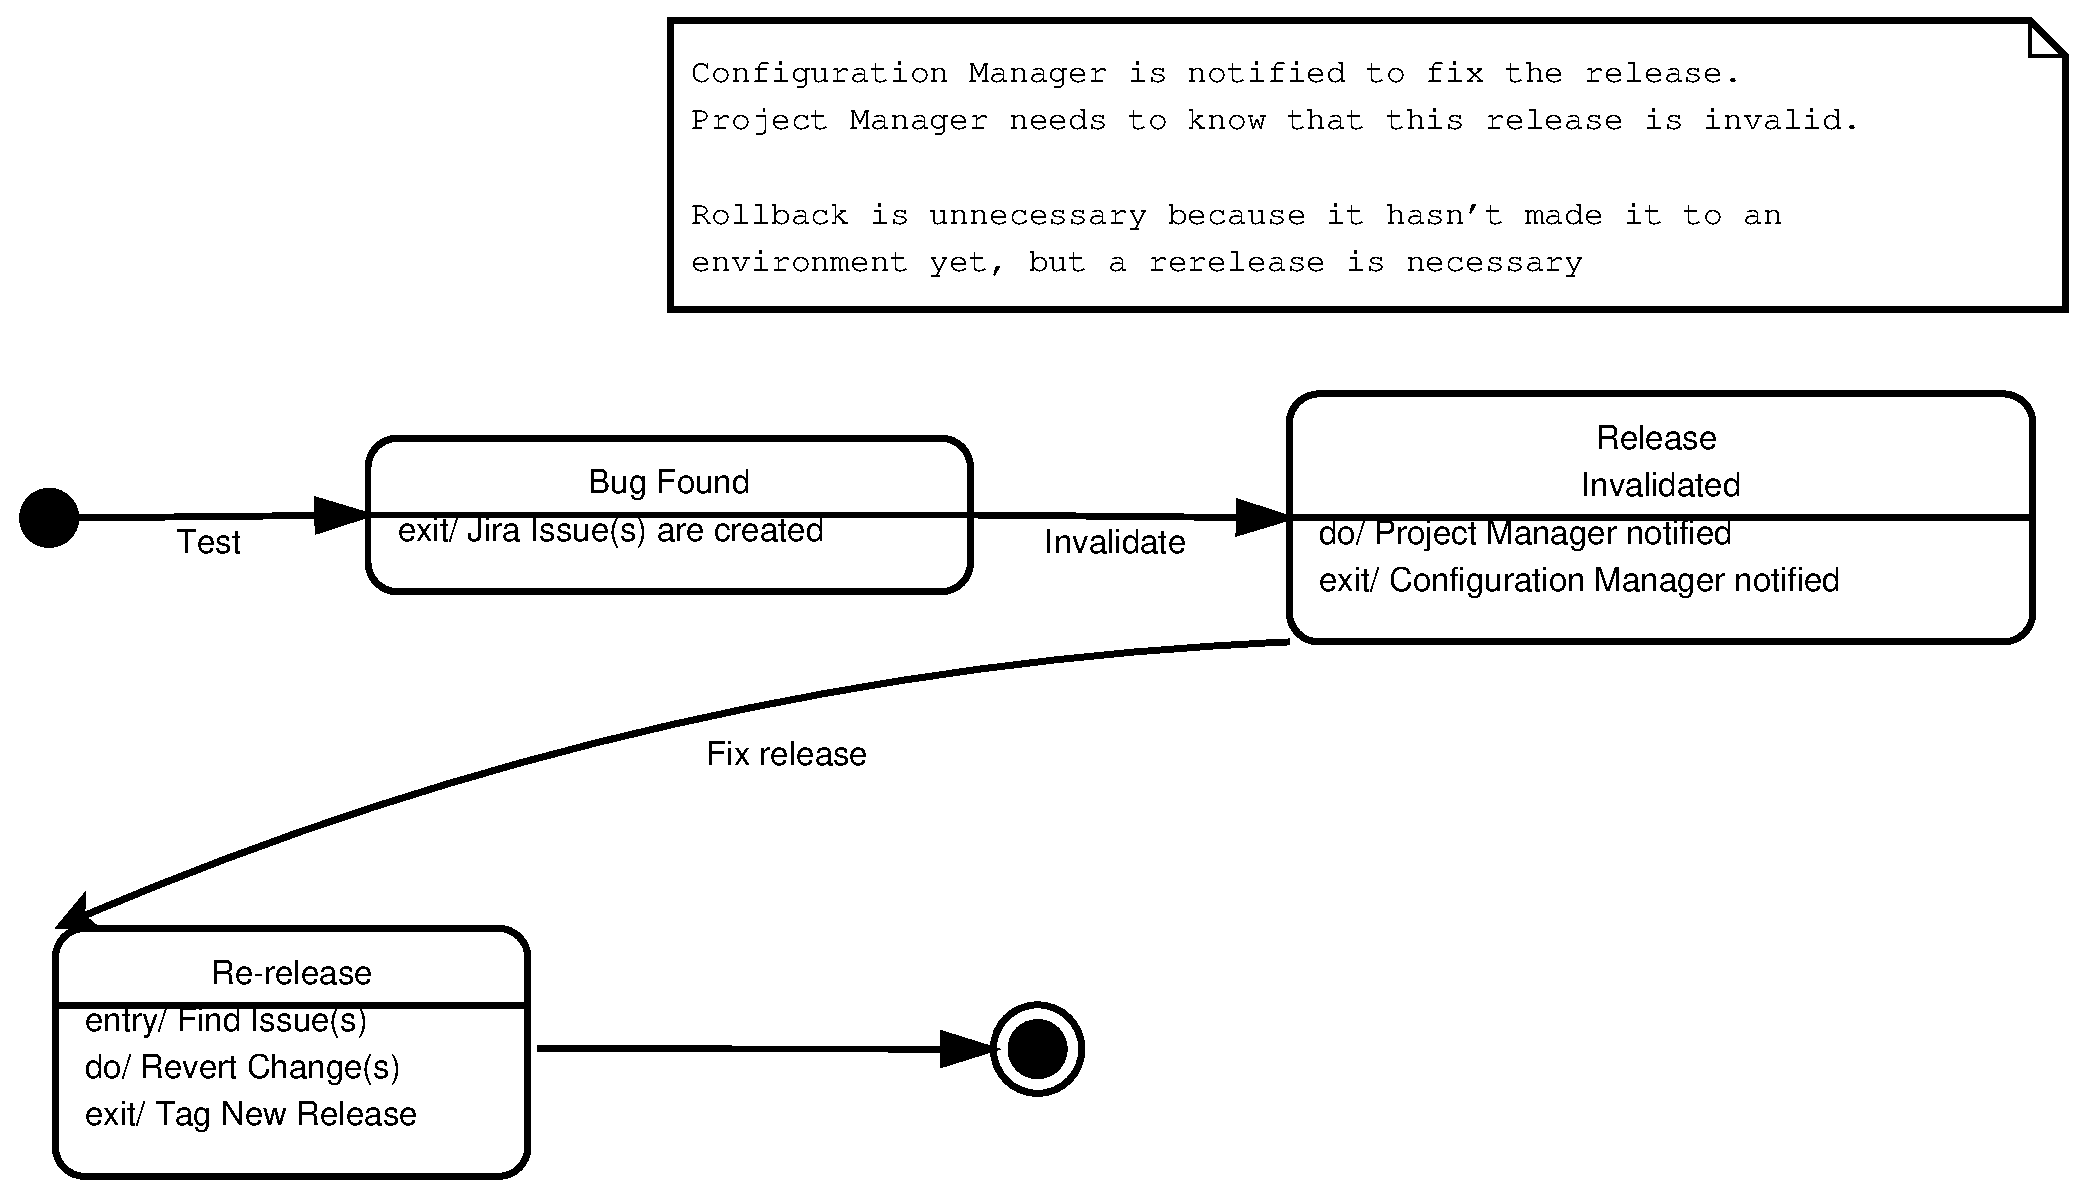
\includegraphics[width=12cm]{Diagrams/ChangePromotion_State6.eps}
\begin{enumerate}
  \item Project Manager notifies Configuration Manager of build failure.
  \item Configuration Manager locates Jira issue related to change.
  \item Configuration Manager merges changes back to the development branch for fixing the bug.
  \item Configuration Manager determines revisions for the change.
  \item Configuration Manager determines files effected by change.
  \item Configuration Manager reverts by revision each file effected. \emph{Note: there are no dependencies
    on files, so we can assume that these files do not effect other changes. }
  \item This is now fixed in the next release that is tagged. \emph{Note: This environment 
  is updated manually, so the Project Manager will have to request another update after the release
  is packaged for this change to get into TST. Meanwhile, TST now functions on a rolledback version.}  
\end{enumerate}

\subsubsection{Steps Contingent on Project Manager Determining Rollback is Necessary}
\begin{enumerate}
  \item Project Manager checks for suitable rollback version by checking jira or remedy for
    the previous version.
  \item Project Manager requests rollback from Environment Specialist
  \item Environment Specialist performs rollback by installing previous version of build.
  \item Project Manager notifies Configuration Manager of build failure.
  \item Configuration Manager locates Jira issue related to change.
  \item Configuration Manager merges changes back to the development branch for fixing the bug.
  \item Configuration Manager determines revisions for the change.
  \item Configuration Manager determines files effected by change.
  \item Configuration Manager reverts by revision each file effected. \emph{Note: there are no dependencies
    on files, so we can assume that these files do not effect other changes. }
  \item This is now fixed in the next release that is tagged. \emph{Note: This environment 
  is updated manually, so the Project Manager will have to request another update after the release
  is packaged for this change to get into TST. Meanwhile, TST now functions on a rolledback version.}  
\end{enumerate}

\subsection{Change Did Not Pass Automated Tests}
In this scenario, Continuous Integration has caught problems before packaging or possibly before tagging.

\subsubsection{Actors}
\emph{These actors are not official roles. That is a person can be considered to
participate in all of these roles. For example, if there is no such thing as a Configuration
Manager in the project, then a Developer may be filling that role. For the sake of
this document, the roles are exclusively identified.}
\begin{itemize}
  \item Developer
\end{itemize}

\subsubsection{Steps}
\begin{enumerate}
\item Developer rolls back change from trunk.
\item Developer fixes change locally.
\item Developer pushes changes back into the trunk.
\end{enumerate}

\emph{Note: When the release has already been tagged following a failure, a package will not be made. Tagging 
happens once per day. I does not happen again except under special circumstances.}

\section{User Testing of Modifications Not in Release Cycle}
Sometimes, it is impractical to put modifications into the release cycle. They may be
buggy, tedious issues that require testing. Still, they are not in the normal release
cycle because they have not gotten technical signoff, peer review, or anything else. It 
is still necessary to test these changes though. One example is KFS 3.1 upgrades. The
solution is a kind of sandbox that allows testers and developers autonomy in the environment.

By not being part of the release cycle, this environment is built normally but from a branch
instead of trunk. Developers can push changes to this branch without a jira release, technical
signoff or anything. This is a sandbox branch, so developers are completely uninhibited from 
commits; however, developers are still responsible for keeping it clean (making sure the 
environment starts without errors.)

\section{Environment Rollback Process}
Outline of the process for handling rollbacks in the case of an exception.
\subsection{Actors}
\emph{These actors are not official roles. That is a person can be considered to
participate in all of these roles. For example, if there is no such thing as a Configuration
Manager in the project, then a Developer may be filling that role. For the sake of
this document, the roles are exclusively identified.}
\begin{itemize}
  \item Project Manager
  \item Environment Specialist
\end{itemize}

\subsection{Steps}
\begin{enumerate}
  \item Project Manager checks Remedy or Jira to determine which version to rollback to.
  \item Project Manager notifies Environment Specialist to rollback to decided version.
  \item Environment Specialist determines what KFS packages are installed in the environment.
  \item Environment Specialist then reinstalls packages to the version determined by the Project Manager. 
    \emph{Note: All KFS packages are downgraded to the package version.}
  \item Environment Specialist notifies Project Manager upon completion.
\end{enumerate}

\end{document}
